% Options for packages loaded elsewhere
% Options for packages loaded elsewhere
\PassOptionsToPackage{unicode}{hyperref}
\PassOptionsToPackage{hyphens}{url}
\PassOptionsToPackage{dvipsnames,svgnames,x11names}{xcolor}
%
\documentclass[
  10pt,
]{article}
\usepackage{xcolor}
\usepackage[margin=2cm]{geometry}
\usepackage{amsmath,amssymb}
\setcounter{secnumdepth}{5}
\usepackage{iftex}
\ifPDFTeX
  \usepackage[T1]{fontenc}
  \usepackage[utf8]{inputenc}
  \usepackage{textcomp} % provide euro and other symbols
\else % if luatex or xetex
  \usepackage{unicode-math} % this also loads fontspec
  \defaultfontfeatures{Scale=MatchLowercase}
  \defaultfontfeatures[\rmfamily]{Ligatures=TeX,Scale=1}
\fi
\usepackage{lmodern}
\ifPDFTeX\else
  % xetex/luatex font selection
\fi
% Use upquote if available, for straight quotes in verbatim environments
\IfFileExists{upquote.sty}{\usepackage{upquote}}{}
\IfFileExists{microtype.sty}{% use microtype if available
  \usepackage[]{microtype}
  \UseMicrotypeSet[protrusion]{basicmath} % disable protrusion for tt fonts
}{}
\makeatletter
\@ifundefined{KOMAClassName}{% if non-KOMA class
  \IfFileExists{parskip.sty}{%
    \usepackage{parskip}
  }{% else
    \setlength{\parindent}{0pt}
    \setlength{\parskip}{6pt plus 2pt minus 1pt}}
}{% if KOMA class
  \KOMAoptions{parskip=half}}
\makeatother
% Make \paragraph and \subparagraph free-standing
\makeatletter
\ifx\paragraph\undefined\else
  \let\oldparagraph\paragraph
  \renewcommand{\paragraph}{
    \@ifstar
      \xxxParagraphStar
      \xxxParagraphNoStar
  }
  \newcommand{\xxxParagraphStar}[1]{\oldparagraph*{#1}\mbox{}}
  \newcommand{\xxxParagraphNoStar}[1]{\oldparagraph{#1}\mbox{}}
\fi
\ifx\subparagraph\undefined\else
  \let\oldsubparagraph\subparagraph
  \renewcommand{\subparagraph}{
    \@ifstar
      \xxxSubParagraphStar
      \xxxSubParagraphNoStar
  }
  \newcommand{\xxxSubParagraphStar}[1]{\oldsubparagraph*{#1}\mbox{}}
  \newcommand{\xxxSubParagraphNoStar}[1]{\oldsubparagraph{#1}\mbox{}}
\fi
\makeatother


\usepackage{longtable,booktabs,array}
\newcounter{none} % for unnumbered tables
\usepackage{calc} % for calculating minipage widths
% Correct order of tables after \paragraph or \subparagraph
\usepackage{etoolbox}
\makeatletter
\patchcmd\longtable{\par}{\if@noskipsec\mbox{}\fi\par}{}{}
\makeatother
% Allow footnotes in longtable head/foot
\IfFileExists{footnotehyper.sty}{\usepackage{footnotehyper}}{\usepackage{footnote}}
\makesavenoteenv{longtable}
\usepackage{graphicx}
\makeatletter
\newsavebox\pandoc@box
\newcommand*\pandocbounded[1]{% scales image to fit in text height/width
  \sbox\pandoc@box{#1}%
  \Gscale@div\@tempa{\textheight}{\dimexpr\ht\pandoc@box+\dp\pandoc@box\relax}%
  \Gscale@div\@tempb{\linewidth}{\wd\pandoc@box}%
  \ifdim\@tempb\p@<\@tempa\p@\let\@tempa\@tempb\fi% select the smaller of both
  \ifdim\@tempa\p@<\p@\scalebox{\@tempa}{\usebox\pandoc@box}%
  \else\usebox{\pandoc@box}%
  \fi%
}
% Set default figure placement to htbp
\def\fps@figure{htbp}
\makeatother





\setlength{\emergencystretch}{3em} % prevent overfull lines

\providecommand{\tightlist}{%
  \setlength{\itemsep}{0pt}\setlength{\parskip}{0pt}}



 


\usepackage{graphicx}
\usepackage{amsmath}
\usepackage{booktabs}
\usepackage{float}
\usepackage{caption}
\usepackage{setspace}
\usepackage{fancyhdr}
\captionsetup{font=small}
\singlespacing
\pagestyle{fancy}
\fancyhf{}
\fancyfoot[C]{\thepage}
\makeatletter
\@ifpackageloaded{caption}{}{\usepackage{caption}}
\AtBeginDocument{%
\ifdefined\contentsname
  \renewcommand*\contentsname{Table of contents}
\else
  \newcommand\contentsname{Table of contents}
\fi
\ifdefined\listfigurename
  \renewcommand*\listfigurename{List of Figures}
\else
  \newcommand\listfigurename{List of Figures}
\fi
\ifdefined\listtablename
  \renewcommand*\listtablename{List of Tables}
\else
  \newcommand\listtablename{List of Tables}
\fi
\ifdefined\figurename
  \renewcommand*\figurename{Figure}
\else
  \newcommand\figurename{Figure}
\fi
\ifdefined\tablename
  \renewcommand*\tablename{Table}
\else
  \newcommand\tablename{Table}
\fi
}
\@ifpackageloaded{float}{}{\usepackage{float}}
\floatstyle{ruled}
\@ifundefined{c@chapter}{\newfloat{codelisting}{h}{lop}}{\newfloat{codelisting}{h}{lop}[chapter]}
\floatname{codelisting}{Listing}
\newcommand*\listoflistings{\listof{codelisting}{List of Listings}}
\makeatother
\makeatletter
\makeatother
\makeatletter
\@ifpackageloaded{caption}{}{\usepackage{caption}}
\@ifpackageloaded{subcaption}{}{\usepackage{subcaption}}
\makeatother
\usepackage{bookmark}
\IfFileExists{xurl.sty}{\usepackage{xurl}}{} % add URL line breaks if available
\urlstyle{same}
\hypersetup{
  pdftitle={Práctica arboles de desición},
  pdfauthor={Ismael Maximiliano De Los Santos Huesca},
  colorlinks=true,
  linkcolor={blue},
  filecolor={Maroon},
  citecolor={Blue},
  urlcolor={Blue},
  pdfcreator={LaTeX via pandoc}}


\title{Práctica arboles de desición}
\author{Ismael Maximiliano De Los Santos Huesca}
\date{2026-10-09}
\begin{document}
\maketitle

\begin{titlepage}

    % Logos alineados izquierda y derecha
    \begin{minipage}{0.45\textwidth}
        \raggedright
        
\includegraphics[width=7cm]{Logo_UNAM.png}
    \end{minipage}
    \hfill
    \begin{minipage}{0.45\textwidth}
        \raggedleft
        
\includegraphics[width=3.4cm]{Logo_LCG.png}
    \end{minipage}

    \centering
    \vspace*{2cm}

    {\Huge\bfseries Práctica arboles de desición \par}
    \vspace{2cm}
    
    {\Large Data Science \par}
    \vspace{1cm}
    
    {\Large De Los Santos Huesca Ismael Maximiliano \par}
    \vspace{1cm}

    {\Large Dr. Carlos Mendez\par}
    \vspace{1cm}
    
    {\Large Fecha: 09 Octubre 2026 \par}
    
    \vfill

\end{titlepage}


\section{Arboles de desición}\label{arboles-de-desiciuxf3n}

Los árboles de decisión son un modelo de aprendizaje supervisado que se
utiliza para clasificación y regresión. Se construyen dividiendo el
conjunto de datos en subconjuntos basados en características.

Para ello, el algoritmo sigue una serie de pasos iterativos en los
cuales se selecciona una característica de manera aleatoria o basada en
una métrica, como la maximización de la entropía. Posteriormente, se
establece un criterio de división basado en esta característica para
dividir el conjunto de datos en dos subconjuntos, que son evaluados en
función de la característica de interés. Este proceso se repite
iterativamente con cada característica seleccionada por el modelo hasta
que todas estén clasificadas.

Esto hace de la fase de entrenamiento un proceso en el que los
hiperparámetros y los datos de entrada juegan un papel importante. En
esta práctica se hará la comparación entre dos tipos de entradas: los
datos escalados y los datos sin escalar, para ver cómo afecta esto a la
predicción del modelo y a sus métricas asociadas.

\subsection{Data}\label{data}

El dataset utilizado para esta tarea corresponde a pacientes con
insuficiencia cardíaca y se encuentra en el archivo
\textbf{heart\_failure\_clinical\_records\_dataset.csv}. Este cuenta con
un total de 13 variables: 12 de ellas son características de los
pacientes y la última es la variable objetivo, que indica si el paciente
falleció o no (203 no y 96 sí), por lo que esta se designa como nuestra
variable de interés a lo largo de las 299 instancias (pacientes) que
componen el dataset.

\subsubsection{Escalamiento}\label{escalamiento}

Para el escalamiento, que es un proceso que normaliza las métricas de
todas las variables con el fin de que tengan la misma escala,
conservando la significancia de las variables categóricas y numéricas,
se utilizó la función \textbf{StandardScaler()} de la librería
\textbf{sklearn.preprocessing}, que estandariza las variables eliminando
la media y escalando a una varianza unitaria.

\subsection{Divisón}\label{divisuxf3n}

El dataset fue dividido en conjuntos de entrenamiento (para ser aplicado
mediante validación cruzada) y prueba de manera aleatoría estratificada
(conservar la proporción real de nuestras clases de interés), a través
de la función \texttt{train\_test\_split} de la librería
\textbf{sklearn.model\_selection}, con un tamaño de prueba del 20 \% y
un random state de 42 para garantizar la reproducibilidad.

{\def\LTcaptype{none} % do not increment counter
\begin{longtable}[]{@{}lrrr@{}}
\toprule\noalign{}
Data-set & Tamaño total & Entrenamiento & Test \\
\midrule\noalign{}
\endhead
\bottomrule\noalign{}
\endlastfoot
Tamaño total & 299 & 239 & 60 \\
Vivo (0) & 203 & 162 & 41 \\
Muerte (1) & 96 & 77 & 19 \\
\end{longtable}
}

\subsection{Entrenamiento}\label{entrenamiento}

Para la selección de hiperparámetros se utilizó la función
\textbf{GridSearchCV()} de la librería
\textbf{sklearn.model\_selection}, que permite realizar una búsqueda
exhaustiva sobre un espacio de hiperparámetros especificado para un
estimador dado mediante validación cruzada. Se evaluaron los parámetros
\texttt{gini} y \texttt{entropy} para el hiperparámetro
\texttt{criterion}, que controla cómo se selecciona iterativamente la
característica para dividir los datos. Para el hiperparámetro
\texttt{class\_weight}, se utilizaron los valores \texttt{balanced},
para la ponderación de clases subrepresentadas, y \texttt{None}.

{\def\LTcaptype{none} % do not increment counter
\begin{longtable}[]{@{}ccc@{}}
\toprule\noalign{}
Modelo & criterion & class\_weight \\
\midrule\noalign{}
\endhead
\bottomrule\noalign{}
\endlastfoot
1 & gini & balanced \\
2 & gini & None \\
3 & entropy & balanced \\
4 & entropy & None \\
\end{longtable}
}

Estos cuatro modelos se entrenaron con datos escalados y sin escalar
mediante validación cruzada de 5 folds, lo que dio un total de 40
entrenamientos y 10 modelos entrenados, de los cuales se eligieron los
mejores de cada tipo de datos utilizados (escalados y sin escalar) para
su evaluación y la obtención de métricas de desempeño.

\subsection{Resultados}\label{resultados}

{\def\LTcaptype{none} % do not increment counter
\begin{longtable}[]{@{}
  >{\raggedright\arraybackslash}p{(\linewidth - 4\tabcolsep) * \real{0.3333}}
  >{\raggedright\arraybackslash}p{(\linewidth - 4\tabcolsep) * \real{0.2963}}
  >{\raggedright\arraybackslash}p{(\linewidth - 4\tabcolsep) * \real{0.3704}}@{}}
\toprule\noalign{}
\begin{minipage}[b]{\linewidth}\raggedright
Métrica
\end{minipage} & \begin{minipage}[b]{\linewidth}\raggedright
Scaled
\end{minipage} & \begin{minipage}[b]{\linewidth}\raggedright
Unscaled
\end{minipage} \\
\midrule\noalign{}
\endhead
\bottomrule\noalign{}
\endlastfoot
\textbf{Hiperparámetros} & \texttt{criterion\ =\ entropy} ·
\texttt{class\_weight\ =\ balanced} & \texttt{criterion\ =\ gini} ·
\texttt{class\_weight\ =\ balanced} \\
F1\_train & 0.634651 & 0.650321 \\
F1\_test & 0.578947 & 0.590909 \\
precision & 0.578947 & 0.52 \\
recall & 0.578947 & 0.684211 \\
roc\_auc & 0.691913 & 0.695764 \\
macro\_F1\_test & 0.691913 & 0.677033 \\
macro\_precision & 0.691913 & 0.674286 \\
macro\_recall & 0.691913 & 0.695764 \\
weighted\_F1\_test & 0.733333 & 0.708612 \\
weighted\_precision & 0.733333 & 0.730857 \\
weighted\_recall & 0.733333 & 0.7 \\
\end{longtable}
}

Se observó que las primeras diferencias surgen como resultado del
entrenamiento en relación con los hiperparámetros seleccionados, siendo
que para los datos escalados se seleccionó el criterio \texttt{entropy}
y para los datos sin escalar se seleccionó el criterio \texttt{gini},
ambos con la ponderación de clases subrepresentadas. Esto nos puede dar
una pauta de comparación para ambos valores del hiperparámetro
\texttt{criterion} y su efecto en las métricas de desempeño, sin dejar
de lado que la comparación también incluye el efecto del escalamiento de
datos en el desempeño del modelo.

Asimismo, el F1 score, aunque similar, parece ser superior en los datos
sin escalar. Esto se conserva en la misma métrica a la hora de la
evaluación, en la que se desarrolla un poco más la causa de esta
diferencia, ya que, aunque la precisión parece ser mayor en el modelo
entrenado con datos escalados, la diferencia se da en el recall, que es
superior en el modelo entrenado con datos sin escalar. Esto nos indica
que este modelo es capaz de identificar un número mayor de verdaderos
positivos, sacrificando su precisión en relación con los falsos
positivos.

En cuanto a las métricas macro y weighted, se observa que el modelo
entrenado con datos escalados es superior en todas ellas. Aun así, las
métricas parecen ser muy similares en ambos modelos, lo que pareciera
tener un efecto discreto en su poder predictivo.

\newpage

\subsubsection{Matriz de confusión}\label{matriz-de-confusiuxf3n}

Por último, se evaluó la matriz de confusión para ambos modelos
@conf-mat:

\begin{figure}[H]

{\centering 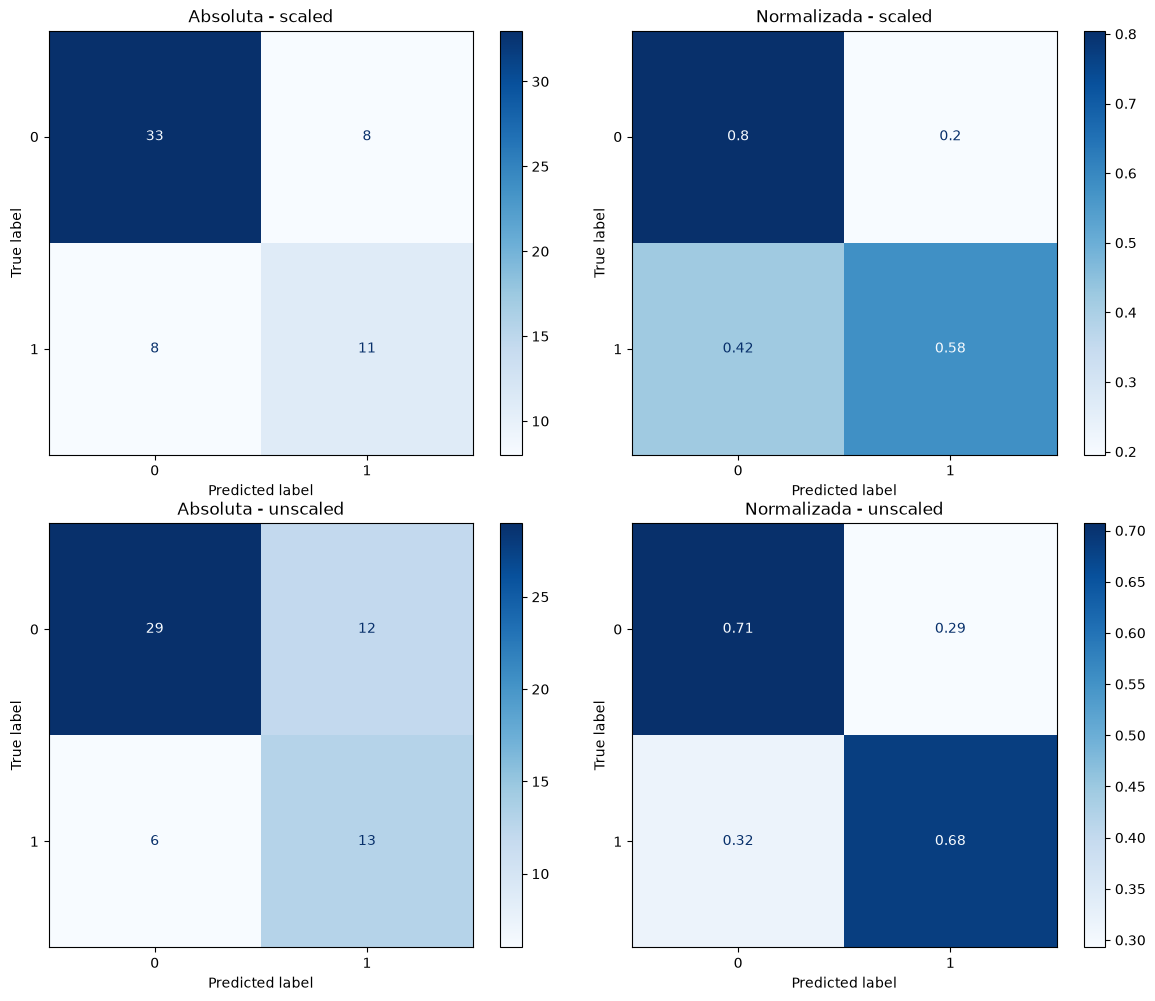
\includegraphics[width=0.85\linewidth,height=\textheight,keepaspectratio]{heart_failure_DT_vGrid.png}

}

\caption{Matriz de confusión}

\end{figure}%

En la matriz de confusión se observa que el modelo entrenado con datos
escalados es capaz, como ya nos anunciaban las métricas, de alcanzar una
precisión mayor que el modelo no escalado. Mientras que el recall para
los datos predichos en la clase 0 de la categoría del evento de muerte
es superior en el modelo escalado, este se pierde para la otra clase
(1), siendo que el modelo sin escalar nos puede dar información más
valiosa, ya que está prediciendo un número mayor de falsos positivos
para la clase 0, lo que puede indicar un posible riesgo de muerte en
pacientes que no lo tienen, pero, a su vez, es capaz de identificar un
mayor número de verdaderos positivos para la clase 1, lo que nos puede
dar una pauta de alerta para pacientes que sí tienen riesgo de muerte.

\subsection{Conclusión}\label{conclusiuxf3n}

En conclusión, se ve un efecto discreto en el uso de datos escalados y
no escalados en el desempeño de ambos modelos, lo que se refleja en las
métricas evaluadas y que, en su formato ponderado, aparenta una
diferencia no significativa entre los mismos en cuanto a su poder
predictivo. Sin embargo, a la hora de evaluar la matriz de confusión, la
información relevante para la pregunta de interés parece decantarse por
el modelo entrenado con datos sin escalar, pudiendo predecir pacientes
en zona de riesgo gracias a su mayor precisión en la clase con evento de
muerte dentro de la misma categoría.

Sin embargo, los valores alcanzados para todas las métricas siguen
siendo relativamente bajos, por lo que futuras estrategias, como
corregir el sesgo en la sobrerrepresentación de la clase 0 en los datos
mediante técnicas de oversampling, podrían ayudar, ya que la reducción
de dimensionalidad o la selección de características parecen ser, a
priori, necesarias para una dimensionalidad de 12 variables (el mismo
análisis profundo del árbol podría revelar el número de variables
utilizadas en su clasificación).

\section{Referencias}\label{referencias}

\begin{enumerate}
\def\labelenumi{\arabic{enumi}.}
\tightlist
\item
  Pedregosa, F., Varoquaux, G., Gramfort, A., Michel, V., Thirion, B.,
  Grisel, O., Blondel, M., Prettenhofer, P., Weiss, R., Dubourg, V.,
  Vanderplas, J., Passos, A., Cournapeau, D., Brucher, M., Perrot, M.,
  \& Duchesnay, E. (2011). Scikit-learn: Machine Learning in Python.
  Journal of Machine Learning Research, 12, 2825--2830.
\end{enumerate}




\end{document}
